\subsection{Uniform distributions and uniform flows}
\begin{itemize}
    \item A uniform flow of degree $g$ and height $h$ is a Markovian flow that models a uniform distribution, meaning all the leaf nodes have the same value. The policy of such flow consists in a function that takes the incoming flow and splits it equally between each of the g outgoing nodes.
\end{itemize}

To start let us consider the example of a flow trained on a uniform distribution and policy that takes the incoming flow and split it equally to all outgoing states. The resulting uniform distribution on the terminal nodes density is  represented by $\pi^*(x)=\frac{1}{g^h}$, for each terminal object in the domain $x \in \mathcal{X}$ and $|\mathcal{X}|=g^h$.

Let us consider the case that the policy at the root of the network introduces an error in the flow of size $\delta$, meaning that one children node now will receive a flow $\frac{F}{g}+\delta$ and the other $g-1$ will continue with $\frac{F}{g}$, which is equivalent to the policy with a probability density (after normalizing) that assigns a probability $\frac{F+g\delta}{g(F+\delta)}$ to one branch and $\frac{F}{g(F+\delta)}$ to the other $g-1$ branches. The total variation distance between this new density and the original policy (uniform probability for each $g$ branches) is $\epsilon(\delta, g)=(1-\frac{1}{g})\frac{\delta}{F+\delta}$. Now we denote the resulting sampling distribution induced by this modified flow as $\pi(x)$.


\begin{figure}[h]
    \center 
% https://q.uiver.app/#q=WzAsMTMsWzMsMCwiRitcXGRlbHRhIl0sWzIsMSwiXFxmcmFje0Z9e2d9K1xcZGVsdGEiXSxbNCwxLCJcXGZyYWN7Rn17Z31cXHRleHR7IH1cXHRyaWFuZ2xlIl0sWzIsMiwiXFx0cmlhbmdsZSJdLFswLDMsIlxcZnJhY3tGfXtnXmh9K1xcZGVsdGFfMSJdLFsxLDIsIlxcdHJpYW5nbGUiXSxbNSwyLCJcXHRyaWFuZ2xlIl0sWzQsMiwiXFx0cmlhbmdsZSJdLFsxLDMsIlxcZnJhY3tGfXtnXmh9K1xcZGVsdGFfMlxcdGV4dHsgIH1cXGxkb3RzICJdLFsyLDMsIlxcZnJhY3tGfXtnXmh9K1xcZGVsdGFfe2dee2gtMX19Il0sWzQsMywiXFxmcmFje0Z9e2deaH0iXSxbNSwzLCJcXGZyYWN7Rn17Z15ofSJdLFs2LDMsIlxcZnJhY3tGfXtnXmh9Il0sWzAsMSwiXFx0ZXh0e2RlZ3JlZSBnfSJdLFswLDJdLFsyLDZdLFsyLDddLFsxLDNdLFsxLDVdLFs1LDRdLFs1LDhdLFszLDldLFs3LDEwXSxbNiwxMV0sWzYsMTJdXQ==
\[\begin{tikzcd}
	&&& {F+\delta} \\
	&& {\frac{F}{g}+\delta} && {\frac{F}{g}\text{ }\triangle} \\
	& \triangle & \triangle && \triangle & \triangle \\
	{\frac{F}{g^h}+\delta_1} & {\frac{F}{g^h}+\delta_2\text{  }\ldots } & {\frac{F}{g^h}+\delta_{g^{h-1}}} && {\frac{F}{g^h}} & {\frac{F}{g^h}} & {\frac{F}{g^h}}
	\arrow["{\text{degree g}}", from=1-4, to=2-3]
	\arrow[from=1-4, to=2-5]
	\arrow[from=2-5, to=3-6]
	\arrow[from=2-5, to=3-5]
	\arrow[from=2-3, to=3-3]
	\arrow[from=2-3, to=3-2]
	\arrow[from=3-2, to=4-1]
	\arrow[from=3-2, to=4-2]
	\arrow[from=3-3, to=4-3]
	\arrow[from=3-5, to=4-5]
	\arrow[from=3-6, to=4-6]
	\arrow[from=3-6, to=4-7]
\end{tikzcd}\]
\caption{A flow network with a extra flow of $\delta$ in one of the branches of the initial state} 
    \label{fig:tree_graph} 
\end{figure}

Let $\mu$ and $\nu$ be two probability measures, then we denote $||\mu - \nu||_{\scaleto{\textbf{TV}}{3pt}}$ as the total variation distance between them. 

\begin{assumption}\label{as: gf_tree_unif}
 Let the pair $(G_T, F)$ be a flow network such that $G_T$ is a regular tree with degree $g$ and depth $h$. Furthermore, assume that $F$ spreads uniformly in the edges of $G_T$, then the target distribution $\pi^*$ generated by $(G_T, F)$ is uniform.      
\end{assumption}

\begin{theorem}[Total variation of the sampling distribution] Let $\delta >0$ and $\sum_{i=1}^{g^{h-1}} \delta_i = \delta$, where $\delta_i \in [0, \delta]$ for all $i \in \{1,2, \dots, g^{h-1}\}$. Suppose that we have the flow network $(G_T, F+\delta)$  abiding by Assumption~\ref{as: gf_tree_unif} besides the first edge from the root to a son where it has a $\delta$ increasing generating a new target distribution $\pi$. Then under these conditions describe the total variation distance between $\pi$ and $\pi^*$ is bounded above and below by the following
\begin{align*}
& \epsilon(\delta, g) \leq ||\pi - \pi^*||_{\scaleto{\textbf{TV}}{3pt}} \leq \epsilon(\delta, g^h) \quad \text{where}
\\
& \epsilon(a,b) := \Big(1 - \frac{1}{b} \Big) \frac{a}{F+a}\,.
\end{align*}
\end{theorem}

\begin{proof}
The terminal states of the modified flow network will have two types of nodes, with flow $\frac{F}{g^h}$ and $\frac{F}{g^h}+\delta_{i}$, with $\delta_i \geq 0$ and $\sum_{i=1}^{g^{h-1}} \delta_i = \delta$. We normalize those probabilities to obtain the individual probabilities for each terminal state, which determines the density of each sample. From that, we can proceed to compute the total variation distance between $\pi$ and $\pi^*$.
\begin{align*}
    ||\pi - \pi^*||_{\scaleto{\textbf{TV}}{3pt}} &= \frac{1}{2}\sum_{x \in \mathcal{X}} | \pi(x)- \pi^*(x) | \\
                          &= \frac{1}{2}\left[(g^h-g^{h-1})\left|\frac{F}{g^h}\frac{1}{F+\delta} - \frac{1}{g^h}\right|+ \sum_{i=1}^{g^{h-1}} \left|\frac{F+g^h\delta_i}{g^h}\frac{1}{F+\delta} - \frac{1}{g^h}\right| \right] \\
                          &= \frac{1}{2}\left[\frac{g^h\delta-g^{h-1}\delta+\sum_{i=1}^{g^{h-1}}|g^h\delta_i-\delta|}{g^h(F+\delta)}\right]
\end{align*}

We can lower bound $\sum_{i=1}^{g^{h-1}}|g^h\delta_i-\delta|$, by considering that $\sum_{i=1}^{g^{h-1}}(g^h\delta_i-\delta)=g^{h}\delta-g^{h-1}\delta$, taking the absolute value of the result and each element of the sum to obtain $g^{h}\delta-g^{h-1}\delta \leq \sum_{i=1}^{g^{h-1}}|g^h\delta_i-\delta|$. Thus we obtain the lower bound 
\begin{align*}
\frac{1}{2}\left[\frac{g^h\delta-g^{h-1}\delta+g^{h}\delta-g^{h-1}\delta}{g^h(F+\delta)}\right]&\leq \frac{1}{2}\left[\frac{g^h\delta-g^{h-1}\delta+\sum_{i=1}^{g^{h-1}}|g^h\delta_i-\delta|}{g^h(F+\delta)}\right] \\
                       \left(1-\frac{1}{g}\right)\frac{\delta}{F+\delta} &\leq  ||\pi - \pi^*||_{\scaleto{\textbf{TV}}{3pt}} 
\end{align*}.

This lower bound is reached when all error terms in the terminal states have the same value $\delta_i = \frac{\delta}{g^h}$.

To upper bound $|g^h\delta_i-\delta|$ we apply the triangle inequality, obtaining $|g^h\delta_i-\delta| \leq g^h\delta_i+\delta$ and  $\sum_{i=1}^{g^{h-1}}|g^h\delta_i-\delta| \leq g^h\delta+g^{h-1}\delta$, from which we obtain the upper bound
\begin{align*}
    ||\pi - \pi^*||_{\scaleto{\textbf{TV}}{3pt}} &\leq \frac{1}{2}\left[\frac{g^h\delta-g^{h-1}\delta + g^{h}\delta+g^{h-1}\delta}{g^h(F+\delta)}\right] \\
    ||\pi - \pi^*||_{\scaleto{\textbf{TV}}{3pt}} &\leq \frac{\delta}{F+\delta}
\end{align*}.

To obtain a tighter bound we break the sum $\sum_{i=1}^{g^{h-1}}|g^h\delta_i-\delta|$ by partitioning the sum into the first $I$ terms $S_A=g^h\sum_{i=1}^{I}|\delta_i-\frac{\delta}{g^h}|$ with $\delta_i < \frac{\delta}{g^h}$ and subsequent $g^{h-1}-I$ terms $S_B=g^h\sum_{j=I+1}^{g^{h-1}}|\delta_j-\frac{\delta}{g^h}|$ with $\delta_j \geq \frac{\delta}{g^h}$. By construction, we know that $S_A+g^h\sum_{i=1}^{I}\delta_i+g^h\sum_{j=I+1}^{g^{h-1}}\delta_j-S_B=g^{h-1}\delta$, simplifying to $S_B-S_A=\delta(g^h-g^{h-1})$. We rewrite $S_A + S_B = S_B-S_A+2S_A=\delta(g^h-g^{h-1})+2S_A$, and by triangle inequality on $S_A$, we obtain the upper bound $\sum_{i=1}^{g^{h-1}}|g^h\delta_i-\delta|=S_A+S_B \leq g^h\delta-g^{h-1}\delta+2I\delta $. Setting $I=g^{h-1}-1$ (the biggest value it can have without breaking the constraints on $\delta_i$), it simplifies to $S_A+S_B \leq g^h\delta+g^{h-1}\delta-2\delta $

\begin{align*}
    ||\pi - \pi^*||_{\scaleto{\textbf{TV}}{3pt}} &\leq \frac{1}{2}\left[\frac{g^h\delta-g^{h-1}\delta+\sum_{i=1}^{g^{h-1}}|g^h\delta_i-\delta|}{g^h(F+\delta)}\right] \\
    ||\pi - \pi^*||_{\scaleto{\textbf{TV}}{3pt}} &\leq \frac{1}{2}\left[\frac{g^h\delta-g^{h-1}\delta+g^h\delta+g^{h-1}\delta-2\delta }{g^h(F+\delta)}\right] \\
    ||\pi - \pi^*||_{\scaleto{\textbf{TV}}{3pt}} &\leq \left[\frac{g^h\delta-\delta }{g^h(F+\delta)}\right] \\
    ||\pi - \pi^*||_{\scaleto{\textbf{TV}}{3pt}} &\leq  \left(1-\frac{1}{g^h}\right)\frac{\delta}{F+\delta}
\end{align*}.
\end{proof}

\textcolor{red}{\begin{theorem}[Total variation of the sampling distribution] Let $\delta >0$ and $\sum_{i=1}^{n} \delta_i = \delta$, where $\delta_i \in [0, \delta]$. Suppose that we have the flow network $(G_n, F)$ which generates a target distribution $\pi^*$ uniform in the number of final vertices. Then if we increase the flow $F$ by $\delta$ in the same graph, that is $(G_n, F + \delta)$, generating a new target distribution $\pi$, the total variation distance between $\pi$ and $\pi^*$ is bounded above and below by the following
\begin{align*}
& ||\pi -\pi^*||_{\scaleto{\textbf{TV}}{3pt}} \leq \epsilon(\delta, n) \quad \text{where}
\\
& \epsilon(a,b) := \Big(1 - \frac{1}{b} \Big) \frac{a}{F+a}\,.
\end{align*}
\end{theorem}}




\section{Inherent limitations of policy networks}



\begin{figure}
    \center 
    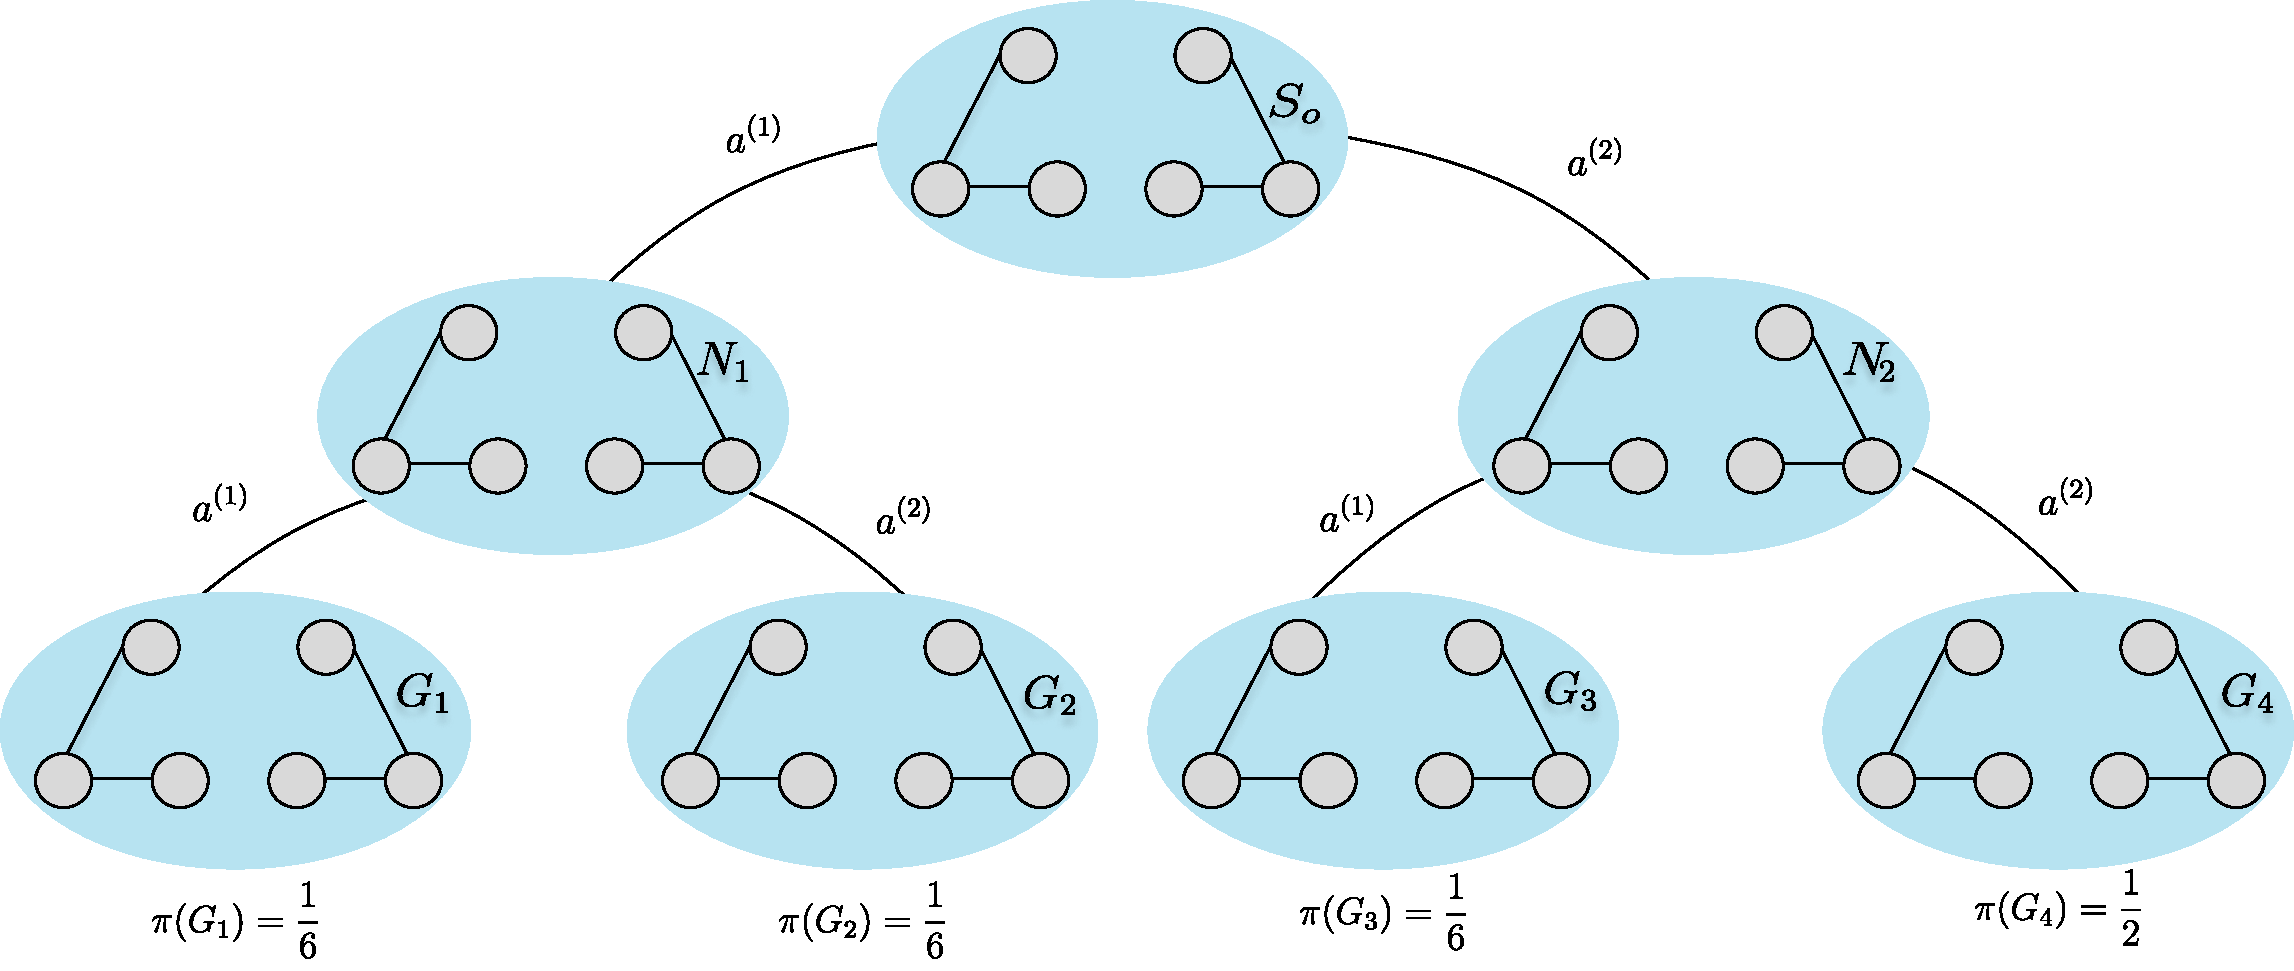
\includegraphics[scale=.3]{gflownets_wl_test.pdf} 
    \caption{A state graph whose downstream distribution is not learnable by a GFlowNet with a policy network is
    parametrized by a 1-WL GNN.} 
    \label{fig:wl_graphs} 
\end{figure}

\begin{theorem}[Distributional constraints of GFlowNets] 
    Let $\mathcal{G} = \{(\mathbf{X}, \mathbf{A}) \colon \mathbf{A} \in \{0,
    1\}^{N \times N}\}$ be the set of equally featured graphs with adjacency matrix $\mathbf{A}$
    and features $\mathbf{r} \in \mathbb{R}^{d}$ ($\mathbf{X} = \mathbf{1}\mathbf{r}^{T} \in \mathbb{R}^{N \times d}$). Let $F_{\theta} \colon \mathcal{G} \rightarrow \Delta_{2}$ be the
    \textit{policy network} that maps a graph $G \in \mathcal{G}$ to a point within the simplex of action-probabilities $\Delta_{2} =
    \{(a^{(1)}, a^{(2)}) \colon a^{(1)} + a^{(2)} = 1 \text{ and
    } a^{(1)}, a^{(2)} \ge 0\}$. See Figure~\ref{fig:wl_graphs}. Suppose that the policy network is parametrized by an 1-WL GNN with parameters $\theta$. Let $\pi$ be a distribution on the
    graphs $\{G_{i} \colon i \in \{1, 2, 3, 4\}\}$ of Figure~\ref{fig:wl_graphs} with $\pi(G_{1}) = \pi(G_{2}) = \pi(G_{3}) =
    \frac{1}{6}$ and $\pi(G_{4}) = \frac{1}{2}$. In these settings, there does not exist a
    $\theta$ such that the downstream distribution induced by the policy network equals $\pi$. 
\end{theorem}

\begin{proof}
    Let $p_{\theta}(X | S_{o})$ be the marginal transition probability learned by the GFlowNet of reaching the state $X
    \in \mathcal{G}$
    through the generative process characterized by the state graph of Figure~\ref{fig:wl_graphs} and the policy network
    $F_{\theta}$. We will show that
    $p_{\theta}(G_{i} | S_{o})$ is -- for any $\theta$ -- necessarily different of $\pi(G_{i})$ for at least two graphs
    in $\pi$'s support. 

    For this, notice that the Markovity of the stochastic transitions learned by the GFlowNet
    entails that 
    $p_{\theta}(G_{1} | S_{o}) = p_{\theta}(N_{1} | S_{o}) p_{\theta}(G_{1} | N_{1})$, 
    $p_{\theta}(G_{2} | S_{o}) = p_{\theta}(N_{1} | S_{o}) p_{\theta}(G_{2} | N_{1})$, 
    $p_{\theta}(G_{3} | S_{o}) = p_{\theta}(N_{2} | S_{o}) p_{\theta}(G_{3} | N_{2})$ and  
    $p_{\theta}(G_{4} | S_{o}) = p_{\theta}(N_{2} | S_{o}) p_{\theta}(G_{4} | N_{2})$. 
    Notably, the indistinguishability of the graphs $N_{1}$ and $N_{2}$ according to the 1-WL 
    isomorphism test implies that $F_{\theta}(N_{1}) = F_{\theta}(N_{2})$ and hence the transition  
    probabilities must satisfy $p_{\theta}(G_{1} | N_{1}) = p_{\theta}(G_{3} | N_{2})$ and $p_{\theta}(G_{2} | N_{1}) =
    p_{\theta}(G_{4} | N_{2})$. 

    Contradictorily, suppose that there is a $\theta$ such that the policy network $F_{\theta}$ is perfectly adjusted to the target distribution $\pi$.
    Hence, $p_{\theta}(G_{i} | S_{o}) = \pi(G_{i})$ for each $i \in \{1, 2, 3, 4\}$. Nonetheless, the representational equivalence of
    $N_{1}$ and $N_{2}$ and the Markovian assumption imply that 

    \begin{equation*} 
        \begin{split} 
        p_{\theta}(N_{1} | S_{o}) = \frac{\pi(G_{1})}{p_{\theta} (G_{1} | N_{1})} 
        = \frac{\pi(G_{3})}{p_{\theta} (G_{3} | N_{2})} = p_{\theta}(N_{2} | S_{o}) 
        \text{ and that } \\ 
        p_{\theta}(N_{1} | S_{o}) = \frac{\pi(G_{2})}{p_{\theta}(G_{2} | N_{1})} \neq 
        \frac{\pi(G_{4})}{p_{\theta}(G_{4} | N_{2})} = p_{\theta}(N_{2} | S_{o}).
        % p_{\theta}(N_{1} | S_{o}) = 
    \end{split} 
    \end{equation*} 

   \noindent This contradiction guarantees that $p(G_{i} | S_{o})$ is necessarily different from $\pi(G_{i})$ for at
   least a pair of graphs and asseverates that the distribution characterized by the state graph of
   Figure~\ref{fig:wl_graphs} is unlearnable by a GFlowNet parametrized by a 1-WL GNN. 
\end{proof}

\begin{remark}
    The previous theorem states the limitations of a GFlowNet parametrized by a 1-WL GNN. The alternative use of a more
    expressive yet not permutationally invariant flow parametrization would entail a factorially large increase of the
    size of the state graph, as equivalent graphs with different labelling would be treated differently by the flow
    estimator, and lead to a computationally untractable problem. The next theorem characterizes a weak relationship
    between the size of the state graph and the statistical efficiency of a maximally entropic exploratory policy within the state graph.   
\end{remark}

\subsubsection*{Author Contributions}
If you'd like to, you may include  a section for author contributions as is done
in many journals. This is optional and at the discretion of the authors.

\subsubsection*{Acknowledgments}
Use unnumbered third level headings for the acknowledgments. All
acknowledgments, including those to funding agencies, go at the end of the paper.
